\section[氢分子]{氢分子} \label{sec:10.04} % 
% \makebox[5em][s]{} % 短题目拉间距

1927年,Heitler-London用量子力学方法研究氢分子结构获得成功,开创了量子化学.

氢分子包含两个原子核$(a,b)$及两个电子$(1,2)$,如图\ref{fig.10-3} 所示.如略去原子核的运动(即分子的振动、转动和平移),就可以将氢分子当作二电子体系,体系的总能量算符可以表示成
\eqllong
\begin{empheq}{align}\label{eqx4.1}
	H=&-\frac{\hbar^{2}}{2m_{e}}(\nabla_{1}^{2}+\nabla_{2}^{2})-\e^{2}(\frac{1}{r_{1a}}+\frac{1}{r_{1b}}+\frac{1}{r_{2a}}+\frac{1}{r_{2b}})+ \nonumber\\
	&\frac{\e^{2}}{r_{12}}+\frac{\e^{2}}{R}
\end{empheq}
\begin{wrapfigure}[7]{r}{8em}
	\centering
	\small
	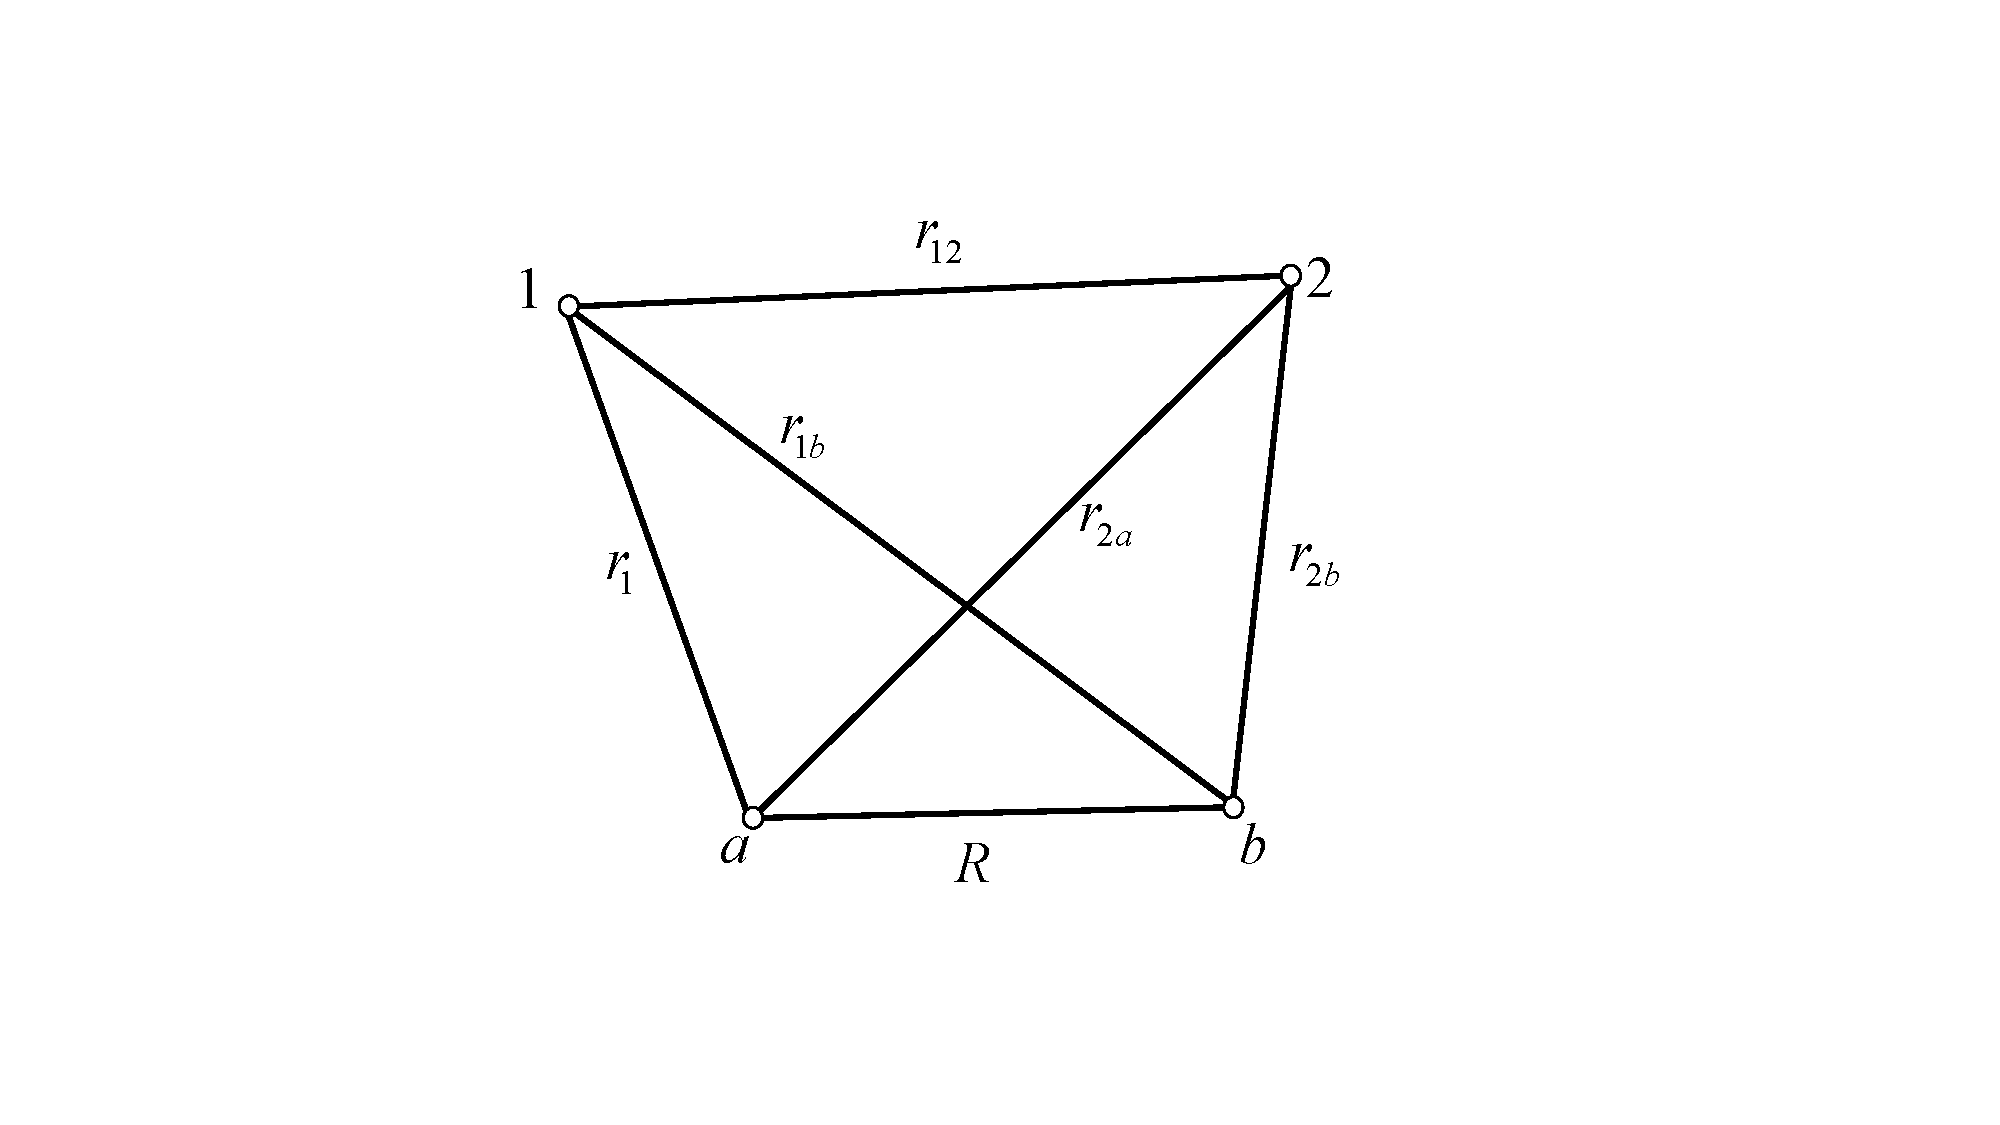
\includegraphics[width=3cm,clip]{QM file/figure/10-3}
	\caption{}\label{fig.10-3}
\end{wrapfigure}
其中共包含6项库仑作用势,最后一项是原子核$a,b$间的库仑能,它是分子能量的一部分,所以应包含在$H$中.在计算中$R$作为参量处理.

和氦原子相仿,二电子体系总波函数可以表示成轨道波函数与自旋波函数的积,
\begin{empheq}{equation}\label{eqx4.2}
	\Psi(q_{1},q_{2})=\varPsi(\boldsymbol{r}_{1},\boldsymbol{r}_{2})\chi(S_{1z},S_{2z})
\end{empheq}\eqnormal
$\varPsi$应满足能量本征方程
\begin{empheq}{equation}\label{eqx4.3}
	H\varPsi(\boldsymbol{r}_{1},\boldsymbol{r}_{2})=E\varPsi(\boldsymbol{r}_{1},\boldsymbol{r}_{2})
\end{empheq}
关于$\varPsi$及$\chi$的交换对称性的讨论以及结论,和氦原子相同,不再重述.由于有两个原子核(即两个库仑力中心),数学处理显然比氦原子更为困难.近似方法通常与物理模型结合使用,大致可分两类,即分子轨函法和原子轨函法.所谓分子轨道是指在原子核$a,b$的库仑场的共同作用下形成的单电子状态,也就是氢分子离子$(\ce{H_{2}^{+}})$的电子轨道态.氢分子的两个电子都处于分子轨道的基态.(自旋态$\chi_{00},S=0$电子间库仑作用$\frac{\e^{2}}{r_{12}}$则作为微扰处理.至于分子轨道波函数的确定仍然要用近似方法(两个库仑力中心!)所谓原子轨道是指孤立原子的单电子状态$\varPsi_{nlm}$.以此作为基础,设法计算两个原子的相互作用能.Heitler-London方法就是原子轨函法,这种方法计算方便,但是精确程度不如分子轨函法.本节只介绍原子轨函法.

考虑分子的形成过程如下:两个孤立的原子逐渐靠近,由于相互作用(电荷间的库仑作用)而结合成分子.以两个原子波函数的积作为分子波函数的零级近似,两原子的相互作用当作微扰.电子与原子核的配对有两种可能,(以每个原子核拥有一个电子为前提,相当于共价键;如二电子同属于一个原子核,就形成离子键.氢分子基本上是共价键类型)如图\ref{fig.10-4}所示,图左相当于原子$(a,2)$与$(b,1)$结合成分子,图右相当于原子$(a,2)$与$(b,1)$结合成分子,两种情形的轨道波函数分别为
\begin{figure}[!h]
	\centering
	\small
	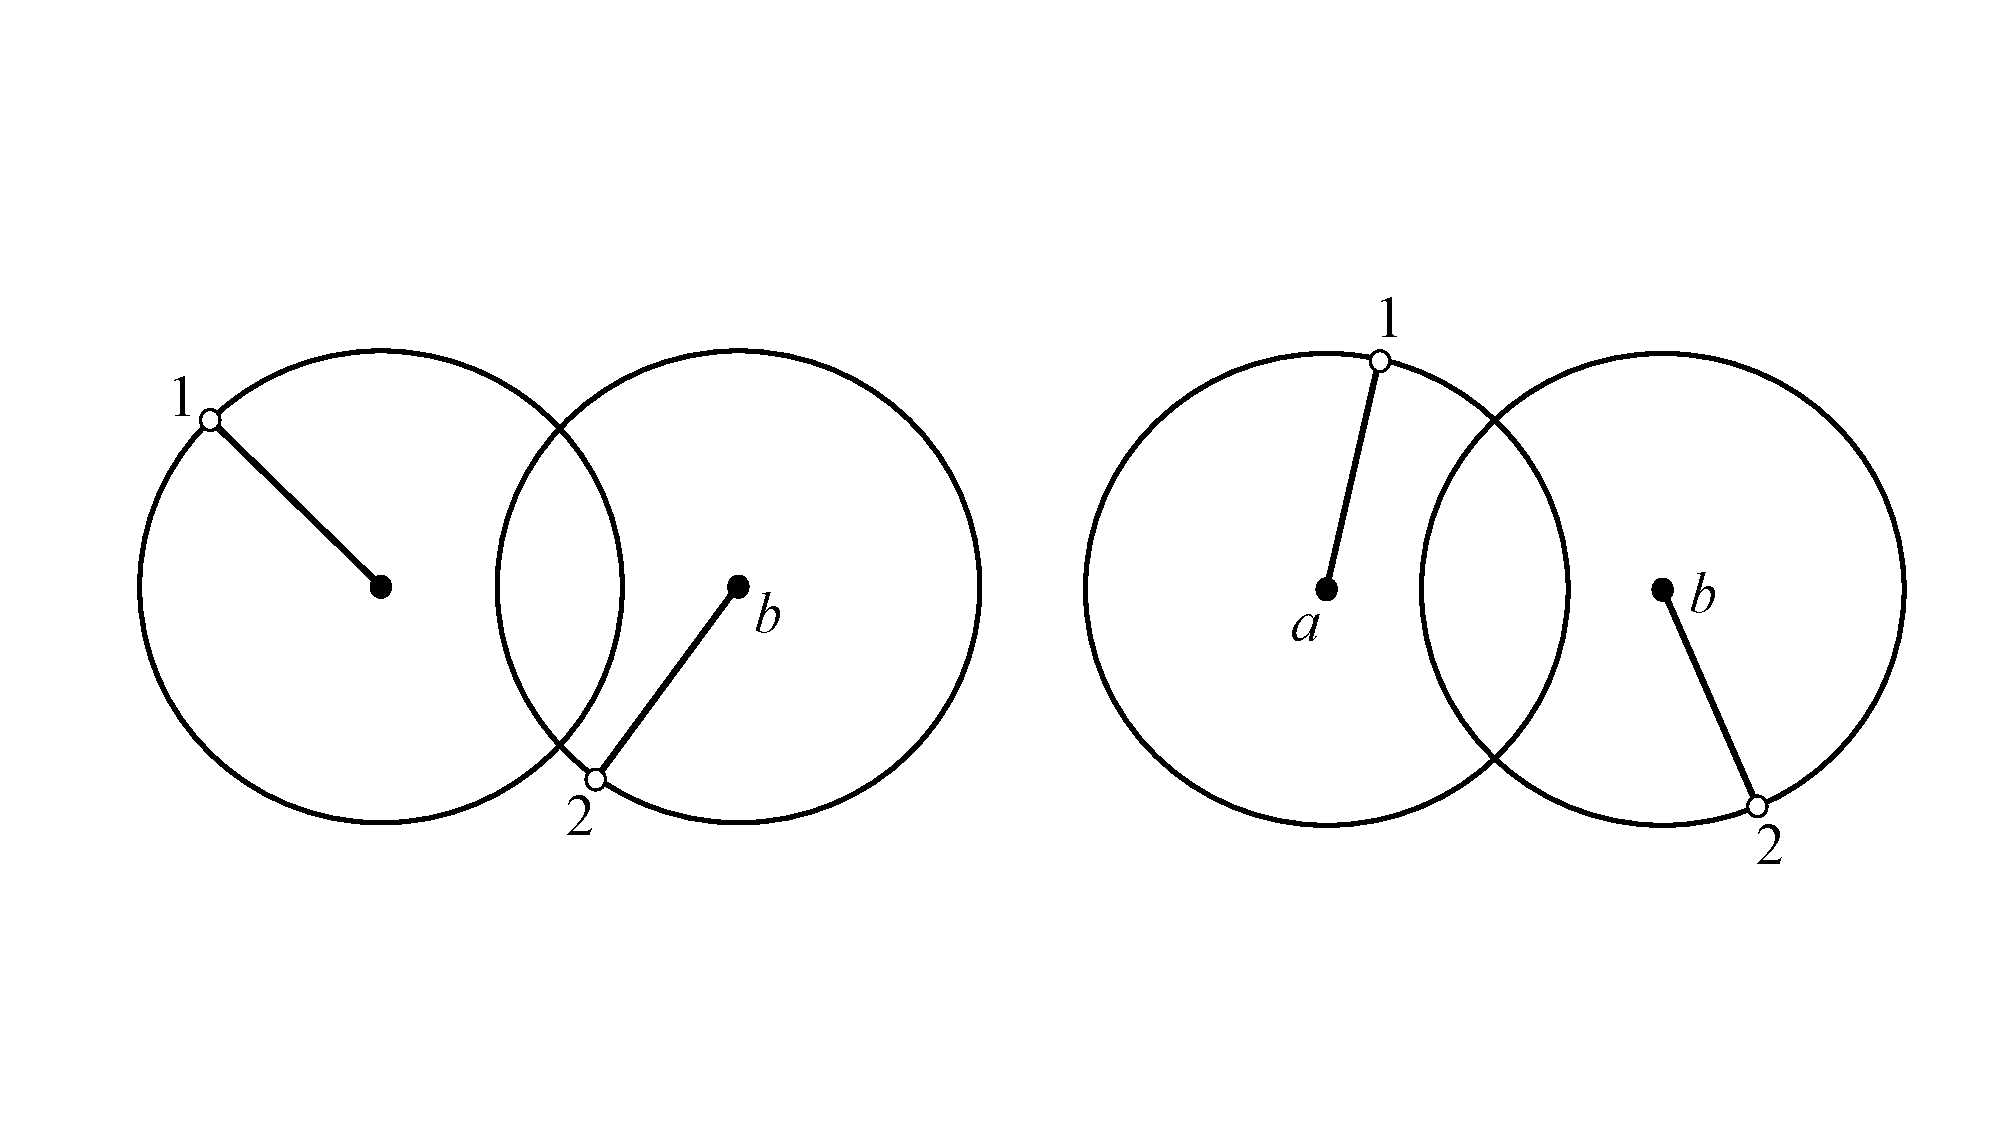
\includegraphics[width=7cm,clip]{QM file/figure/10-4}
	\caption{}\label{fig.10-4}
\end{figure}
\begin{empheq}{equation}\label{eqx4.4}
	\varPsi_{a}(1)\varPsi_{b}(2),\quad \varPsi_{a}(2)\varPsi_{b}(1)
\end{empheq}
其中$\varPsi_{a}(1)$指氢原子$(a,1)$的基态波函数,即
\begin{empheq}{equation}\label{eqx4.5}
	\varPsi_{a}(1)=\varPsi_{100}(r_{1a})=\left(\frac{1}{\pi a_{0}^{3}}\right)^{\frac{1}{2}}e^{-r_{1a}/a_{0}}
\end{empheq}
依此类推.将总能$H$分成$H_{0}$和$H^{\prime}$,$H_{0}$是与两个氢原子的构成有关的算符,$H^{\prime}$是两个原子的相互作用能.对于\eqref{eqx4.4}式中第一个波函数$\varPsi_{a}(1)\varPsi_{b}(2)$,$H_{0}$与$H^{\prime}$分别是
\begin{empheq}{equation}\label{eqx4.6}
	\begin{aligned}
		H_{0} &=-\frac{\hbar^{2}}{2m_{e}}(\nabla_{1}^{2}+\nabla_{2}^{2})-\frac{\e^{2}}{r_{1a}}-\frac{\e^{2}}{r_{1b}}	\\
		H^{\prime} &=\frac{\e^{2}}{R}+\frac{\e^{2}}{r_{12}}-\frac{\e^{2}}{r_{1b}}-\frac{\e^{2}}{r_{2a}}
	\end{aligned}
\end{empheq}
显然
\begin{empheq}{equation*}
	H_{0}\varPsi_{a}(1)\varPsi_{b}(2)=2E_{1}\varPsi_{a}(1)\varPsi_{b}(2),\quad E_{1}=-\frac{\e^{2}}{2a_{0}}
\end{empheq}
$E_{k}$是氢原子基态能级.对于\eqref{eqx4.4}式中第二个波函数$\varPsi_{a}(2)\varPsi_{a}(1)$,$H_{0}$与$H^{\prime}$应取
\begin{empheq}{equation*}\label{eqx4.6'}
	\begin{aligned}
		H_{0} &=-\frac{\hbar^{2}}{2m_{e}}(\nabla_{1}^{2}+\nabla_{2}^{2})-\frac{\e^{2}}{r_{1b}}-\frac{\e^{2}}{r_{2a}}	\\
		H^{\prime} &=\frac{\e^{2}}{R}+\frac{\e^{2}}{r_{12}}-\frac{\e^{2}}{r_{1a}}-\frac{\e^{2}}{r_{2b}}
	\end{aligned}\tag{$10.4.6^{\prime}$}
\end{empheq}
显然
\begin{empheq}{equation*}
	H_{0}\varPsi_{a}(2)\varPsi_{b}(1)=2E_{1}\varPsi_{a}(2)\varPsi_{b}(1)
\end{empheq}\eqlong

如果不管波函数的交换对称性,简单地以\eqref{eqx4.4}式中任何一个(例如第一个)波函数$\varPsi_{a}(1)\varPsi_{b}(2)$作为分子的近似波函数,而以$H^{\prime}$平均值当作分子的结合能,记为$W$,则
\begin{empheq}{equation}\label{eqx4.7}
	W=\iint\varPsi_{a}^{2}(1)\varPsi_{b}^{2}\left(\frac{\e^{2}}{R}+\frac{\e^{2}}{r_{12}}-\frac{\e^{2}}{r_{1b}}-\frac{\e^{2}}{r_{2a}}\right)e^{-2R/a_{0}}
\end{empheq}
$W$之值显然与$R$有关,计算结果为
\begin{empheq}{equation}\label{eqx4.8}
	W=\frac{\e^{2}}{a_{0}}\left(\frac{a_{0}}{R}+\frac{5}{8}-\frac{3}{4}\frac{R}{a_{0}}-\frac{1}{6}\frac{R^{2}}{a_{0}^{2}}\right)e^{-2R/a_{0}}
\end{empheq}
当$R=1.87 a_{0}$时$W$取极小值,
\begin{empheq}{equation}\label{eqx4.9}
	W(R=1.87 a_{0})=-\num{0.0196}\left(\frac{\e^{2}}{a_{0}}\right)=-\num{0.533}\si{eV}.
\end{empheq}\eqnormal
而氢分子结合能的实验值是\num{-4.72}\si{eV},键长$R=\num{0.07395}\si{nm}$.\eqref{eqx4.9}式与实验值相差太多,量级不符合,由此可见,如不考虑波函数的交换对称性,就不能解释氢分子的形成.

考虑到交换对称性,氢分子轨道波函数(零级近似)应取\eqref{eqx4.4}式中两项的对称或反对称组合.以$\varPsi_{ab}^{S}(\boldsymbol{r}_{1},\boldsymbol{r}_{2})$和$\varPsi_{ab}^{A}(\boldsymbol{r}_{1},\boldsymbol{r}_{2})$表示对称和反对称轨道波函数,它们是
\begin{empheq}{align}
	\varPsi_{ab}^{S} &=C_{S}[\varPsi_{a}(1)\varPsi_{b}(2)+\varPsi_{a}(2)\varPsi_{b}(1)]	\label{eqx4.10}\\
	\varPsi_{ab}^{A} &=C_{A}[\varPsi_{a}(1)\varPsi_{b}(2)-\varPsi_{a}(2)\varPsi_{b}(1)]	\label{eqx4.11}
\end{empheq}
$C_{S}$及$C_{A}$是归一化常数.由于叠加的两个波函数并不正交,$C_{S}$及$C_{A}$均不等于$\frac{1}{\sqrt{2}}$.原子轨道波函数$\varPsi_{a}(1)$等已经归一化.定义重叠积分
\begin{empheq}{align}\label{eqx4.12}
	D 	&=\int\varPsi_{a}(1)\varPsi_{b}(1)d\tau_{1}	\nonumber\\
		&=\frac{1}{\pi a_{0}^{3}}\int e^{-(r_{1a}+r_{1b})/a_{0}}d\tau_{1}	\nonumber\\
		&=\left(1+\frac{R}{a_{0}}+\frac{1}{3}\frac{R^{2}}{a_{0}^{2}}\right)e^{-R/a_{0}}
\end{empheq}
则
\begin{empheq}{equation}\label{eqx4.13}
	C_{S}^{2}=\frac{1}{2+2D^{2}},\quad C_{A}^{2}=\frac{1}{2-2D^{2}}
\end{empheq}
当$R\rightarrow0$,原子核$a,b$重合,$\varPsi_{a}=\varPsi_{b}$,$D\rightarrow1$.当$R\rightarrow\infty$,$\varPsi_{a}$与$\varPsi_{b}$完全不重叠,$D\rightarrow0$.用本节所述方法处理氢分子构造,所得键长$R=\num{0.08}\si{nm}=\num{1.518}a_{0},D=\num{0.72},D^{2}=\num{0.52}$.

对于\eqref{eqx4.10}、\eqref{eqx4.11}式分别计算$H^{\prime}$平均值,分别记为$V_{ab}^{S},V_{ab}^{A}$,则可算出
\begin{empheq}{align}
	V_{ab}^{S} &=\iint\varPsi_{ab}^{S}H^{\prime}\varPsi_{ab}^{S}d\tau_{1}d\tau_{2}	\nonumber\\
	&=\frac{W+J}{1+D^{2}}	\label{eqx4.14}\\
	V_{ab}^{A} &=\iint\varPsi_{ab}^{A}H^{\prime}\varPsi_{ab}^{A}d\tau_{1}d\tau_{2}	\nonumber\\
	&=\frac{W-J}{1-D^{2}}		\label{eqx4.15}
\end{empheq}\eqindent{1}
计算时$H^{\prime}$应视作用的对象而取\eqref{eqx4.6}式或\eqref{eqx4.6'}式.$W$由\eqref{eqx4.8}式表示,$J$由下式表示,
\begin{empheq}{align}\label{eqx4.16}
	J	&=\iint\varPsi_{a}(1)\varPsi_{b}(2)\left(\frac{\e^{2}}{R}+\frac{\e^{2}}{r_{12}}-\frac{\e^{2}}{r_{1a}}-\frac{\e^{2}}{r_{2b}}\right)\varPsi_{a}(2)\varPsi_{b}(1)d\tau_{1}d\tau_{2}	\nonumber\\
	&=\varPsi_{a}(2)\varPsi_{b}(1)\left(\frac{\e^{2}}{R}+\frac{\e^{2}}{r_{12}}-\frac{\e^{2}}{r_{1b}}-\frac{\e^{2}}{r_{2a}}\right)\varPsi_{a}(1)\varPsi_{b}(2)d\tau_{1}d\tau_{2}	
\end{empheq}\eqnormal
$W$的意义是两个电子各自占有确定的原子轨道时两个原子间的库仑作用平均值,通常称为库仑能.$J$的意义则是“交换能”,它仍来自两原子间的库仑作用,是电子波函数交换对称性的产物.$J$的计算相当复杂,结果无法用初等解析函数表示.数值计算表明,$V_{ab}^{S}$与$V_{ab}^{A}$都是$R$的函数,$V_{ab}^{S}$在$R=\num{1.518}a_{0}$处有极小值,$W$与$J$均为负值,但$|J|\gg|W|$,数值为
\begin{empheq}{equation*}
	V_{ab}^{S}=\frac{W+J}{1+D^{2}}=-\num{0.125}\left(\frac{\e^{2}}{a_{0}}\right)=-3.41\si{eV}
\end{empheq}
与氢分子结合能实验值$(-4.72\si{eV})$量级符合.由此可知,波函数的交换对称性及“交换能”对于氢分子的形成起了关键作用.其他的共价键分子,也是这样.总之,共价键分子的形成是与全同性原理有关的一种典型量子力学效应,不可能在经典物理或玻尔量子论的基础上予以解释.

由于$|J|\gg|W|,J<0$,所以$V_{ab}^{A}>0$,亦即\eqref{eqx4.11}式所描述的反对称轨道态不能使两原子结合成分子.氢分子的轨道状态近似地由\eqref{eqx4.10}式表示,它是对称态与此相关,氢分子中两个电子的自旋态必为反对称态$\chi_{00}$,总自旋$S=0$,这一点与实验结果完全一致.

$W,V_{ab}^{S},V_{ab}^{A}$随$R$的变化示意图如图\ref{fig.10-5}所示.

\begin{figure}[!h]
	\centering
	\small
	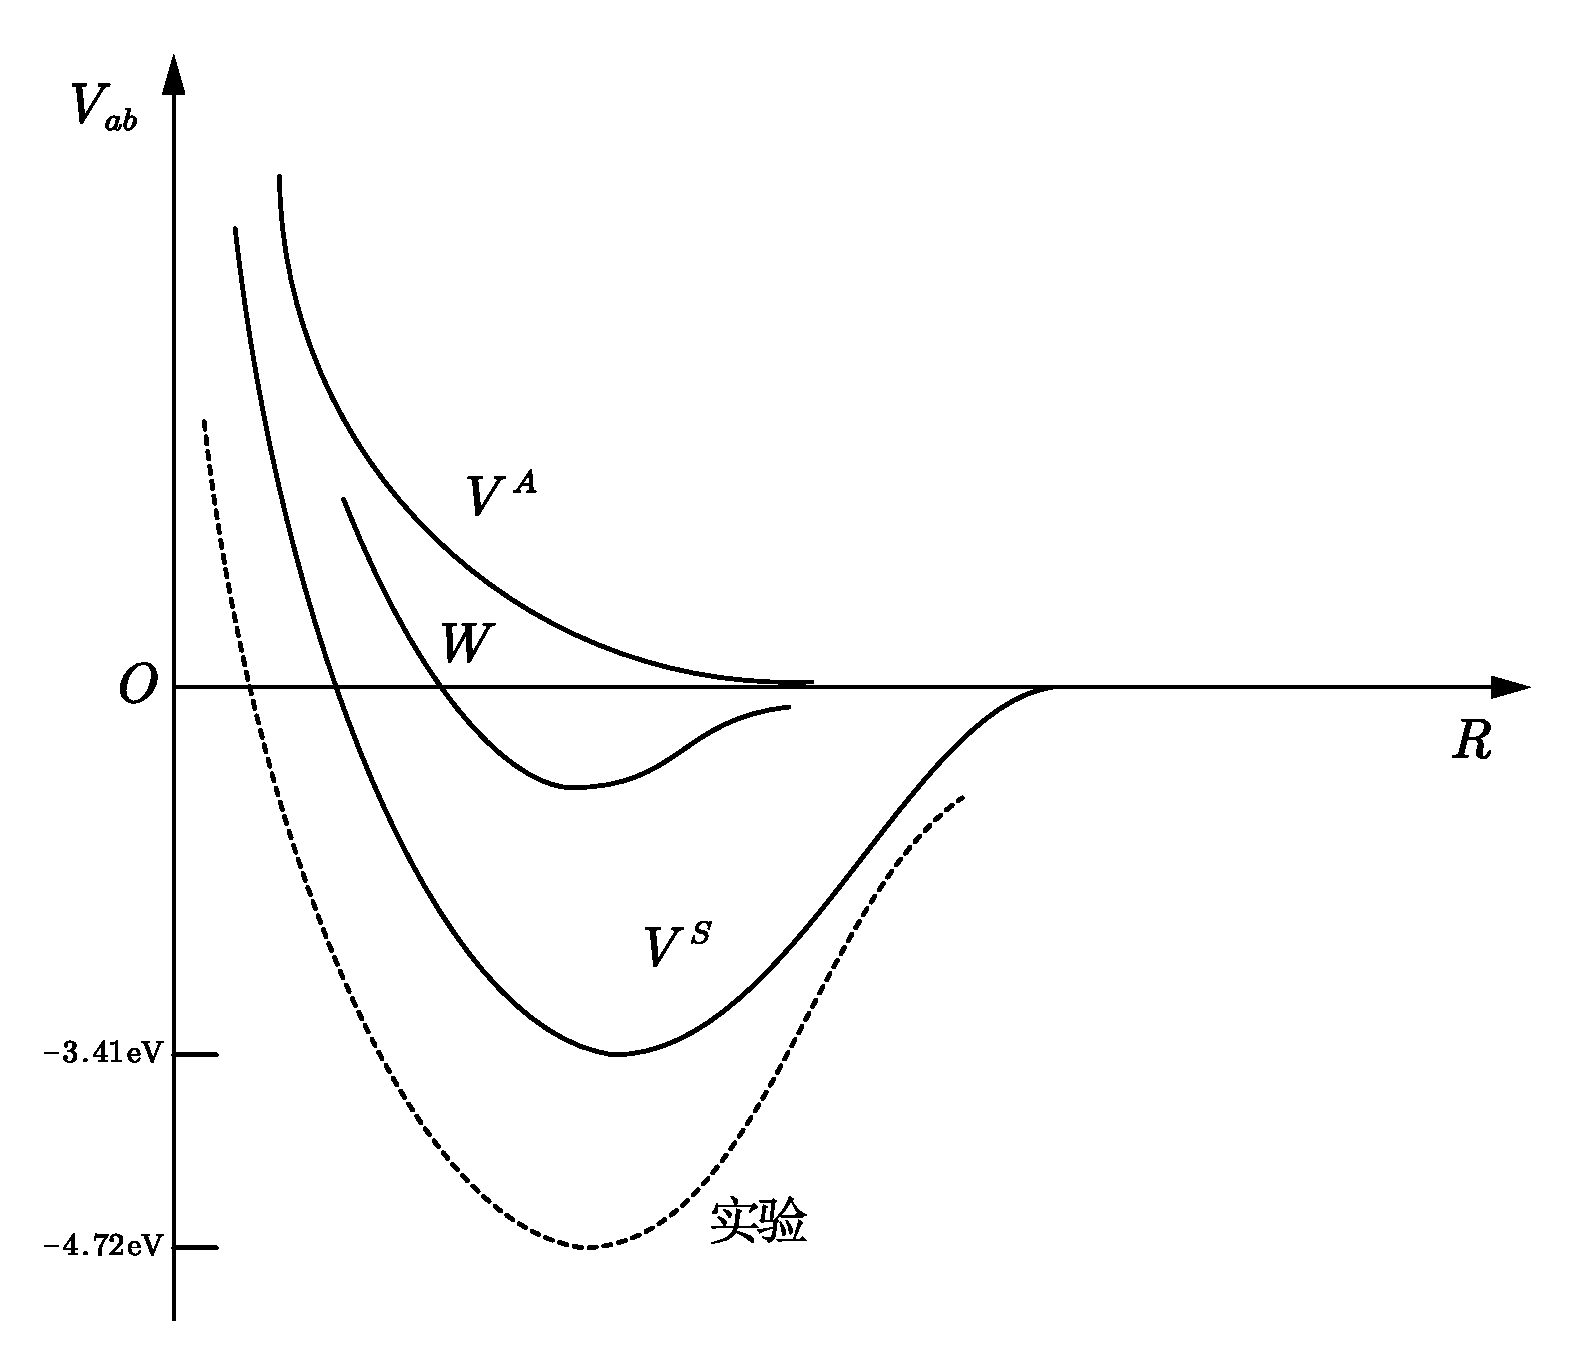
\includegraphics[width=5.5cm,clip]{QM file/figure/10-5}
	\caption{}\label{fig.10-5}
\end{figure}
\begin{wrapfigure}[7]{r}{7em}
	\centering
	\small
	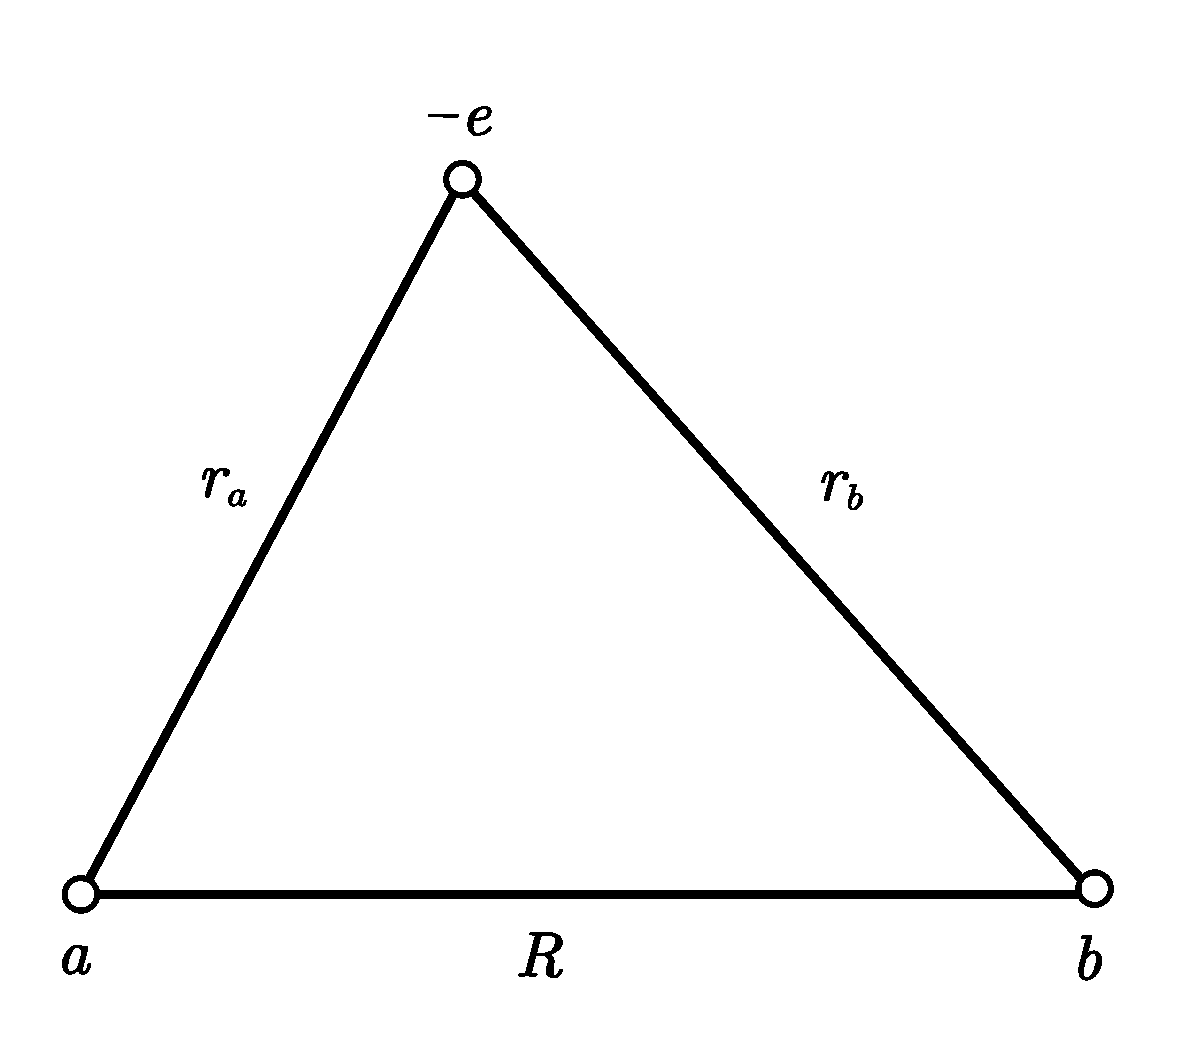
\includegraphics[width=3cm,clip]{QM file/figure/10-6}
	\caption{}\label{fig.10-6}
\end{wrapfigure}
詹姆斯等在考虑交换对称性的前提下,用变分法计算氢分子结合能.他们采用十分复杂的(包含13个变分参数)试探波函数,终于算出与实验值完全一致的结合能.

这表明分子的构造完全受量子力学规律支配,并没有任何超物理的因素起作用.

附录:重叠积分$D$和“库仑能”$W$的计算.

重叠积分$D$的定义见\eqref{eqx4.12}式,略去下标1,$D$可以写成
\begin{empheq}{equation*}
	D=\frac{1}{\pi a_{0}^{3}}\int e^{-(r_{a}+r_{b})/a_{0}}d\tau
\end{empheq}
$r_{a}$及$r_{b}$为电子至核$a$及核$b$之距离,如图10-6所示.引入共焦椭球坐标$(\xi,\eta,\varphi)$,定义为:
\begin{empheq}{align}\label{eqx4.17}
	\xi &=\frac{1}{R}(r_{a}+r_{b}),\quad 1\leqslant\xi <\infty	\\
	\eta&=\frac{1}{R}(r_{a}-r_{b}),\quad -1\leqslant\eta\leqslant1	\nonumber\\
	\varphi&\text{为绕ab轴的旋转角},0\leqslant\varphi <2\pi	\nonumber
\end{empheq}
体积元$d\tau$可以表示成
\begin{empheq}{equation}\label{eqx4.18}
	d\tau=\frac{R^{3}}{8}(\xi^{2}-\eta^{2})d\xi d\eta d\varphi
\end{empheq}
$r_{a},r_{b}$可以表示成
\begin{empheq}{equation}\label{eqx4.19}
	r_{a}=\frac{R}{2}(\xi+\eta),\quad r_{b}=\frac{R}{2}(\xi-\eta)
\end{empheq}\eqindent{5}
代入$D$中,即可算出
\begin{empheq}{align}\label{eqx4.20}
	D 
	&=\frac{1}{8\pi}\left(\frac{R}{a_{0}}\right)^{3}\int_{0}^{2\pi}d\varphi\int_{1}^{\infty}d\xi\int_{-1}^{1}d\eta(\xi^{2}-\eta^{2})e^{-\xi R/a_{0}}	\nonumber\\
	&=\frac{1}{4}\left(\frac{R}{a_{0}}\right)^{3}\int_{1}^{\infty}(2\xi^{2}-\frac{2}{3})e^{-\xi R/a_{0}}d\xi	\nonumber\\
	&=\left(1+\frac{R}{a_{0}}+\frac{1}{3}\frac{R^{2}}{a_{0}^{2}}\right)e^{-R/a_{0}}=D(R,a_{0})
\end{empheq}\eqnormal
此即\eqref{eqx4.12}式.积分的最后一步可用分部积分法算出.

“库仑能”$W$的定义见\eqref{eqx4.7}式.由于$\varPsi_{a}(1),\varPsi_{b}(2$均已归一化,显然
\begin{empheq}{equation*}
	\iint\varPsi_{a}^{2}(1)\varPsi_{b}^{2}(2)\frac{\e^{2}}{R}d\tau_{1}d\tau_{2}=\frac{\e^{2}}{R}
\end{empheq}\eqindent{5}
\begin{empheq}{align}\label{eqx4.21}
	&\iint\varPsi_{a}^{2}(1)\varPsi_{b}^{2}(2)\frac{1}{r_{1b}}d\tau_{1}d\tau_{2}
	=\iint\varPsi_{a}^{2}(1)\varPsi_{b}^{2}(2)\frac{1}{r_{2a}}d\tau_{1}d\tau_{2}	\nonumber\\
	&=\int\varPsi_{b}^{2}(2)\frac{1}{r_{2a}}d\tau_{2}=\frac{1}{\pi a_{0}^{3}}\int\frac{1}{r_{a}}e^{-2r_{b}/a_{0}}d\tau	\nonumber\\
	&=\frac{R^{3}}{4\pi a_{0}^{3}}\iiint d\xi d\eta d\varphi(\xi-\eta)e^{-(\xi-\eta)R/a_{0}}	\nonumber\\
	&=\frac{1}{R}-\left(\frac{1}{R}+\frac{1}{a_{0}}\right)e^{-2R/a_{0}}=I_{1}
\end{empheq}\eqnormal
\eqref{eqx4.7}式中较难的积分是
\begin{empheq}{equation}\label{eqx4.22}
	I_{2}=\iint\varPsi_{a}^{2}(1)\varPsi_{b}^{2}(2)\frac{1}{r_{12}}d\tau_{1}d\tau_{2}
\end{empheq}
先对d$\tau_{1}$积分,用普通球坐标,以原子核$a$作为坐标原点,对角度的积分仿照$\S$\ref{sec:10.03}曾用过的方法,$\frac{1}{r_{12}}$的积分效果相当于$\frac{1}{r_{2a}}$(当$r_{1a}<r_{2a}$)或$\frac{1}{r_{1a}}$(当$r_{2a}<r_{1a}$),因此
\begin{empheq}{align*}
	&\int\varPsi_{a}^{2}(1)\frac{d\tau_{1}}{r_{12}}=\frac{1}{\pi a_{0}^{3}}\int\frac{d\tau_{1}}{r_{12}}e^{-2r_{1a}/a_{0}}	\nonumber\\
	=&\frac{4}{a_{0}^{3}}\left[\frac{1}{r_{2a}}\int_{0}^{r_{2a}}drr^{2}e^{-2r/a_{0}}+\int_{r_{2a}}^{\infty}drre^{-2r/a_{0}}\right]
\end{empheq}
用分部积分法不难算出这二个积分,代入$I_{2}$中,整理后,可得
\begin{empheq}{equation*}\label{eqx4.22'}
	I_{2}=I_{1}-\frac{1}{8a_{0}}D\left(R,\frac{a_{0}}{2}\right)-I_{3}	\tag{$10.4.22^{\prime}$}
\end{empheq}
$D\left(R,\frac{a_{0}}{2}\right)$表示\eqref{eqx4.20}式中$a_{0}\rightarrow\frac{a_{0}}{2}$.$I_{3}$是下列积分:
\begin{empheq}{align}\label{eqx4.23}
	I_{3} &=\frac{1}{\pi a_{0}^{3}}\int\frac{d\tau}{r_{a}}e^{-2(r_{a}+r_{b})/a_{0}}	\nonumber\\
	&=\frac{R^{2}}{4\pi a_{0}^{3}}\iiint d\xi d\eta d\varphi(\xi-\eta)e^{-2\xi R/a_{0}}	\nonumber\\
	&=\frac{1}{4}\left(\frac{1}{a_{0}}+\frac{2R}{a_{0}^{2}}\right)e^{-2R/a_{0}}
\end{empheq}\eqlong
代入\eqref{eqx4.22'}式,即得
\begin{empheq}{equation}\label{eqx4.24}
	I_{2}=\frac{1}{R}-\frac{1}{R}\left(1+\frac{11R}{8a_{0}}+\frac{3R^{2}}{4a_{0}^{2}}+\frac{R^{3}}{6a_{0}^{3}}\right)e^{-2R/a_{0}}
\end{empheq}\eqnormal
以上结果代入\eqref{eqx4.7}式,即得\eqref{eqx4.8}式.

